\documentclass[tikz,border=10pt]{article}
\usepackage{amsmath}
\usepackage{comment}
%\usetikzlibrary{arrows.meta}
\usepackage{pgfplots}
\usepgfplotslibrary{fillbetween}
\usetikzlibrary{fadings}
\tikzfading[name=myfading, bottom color=transparent!100, top color=transparent!0]

\begin{document}
\begin{comment}
\begin{tikzpicture}[
    x                = 2cm/10,
    scale            = 3,
    axis/.style      = {help lines, -{Stealth[length = 1.5ex]}},
    brillouin/.style = {domain = -5:10, samples = 100}
  ]
  %\draw [axis] (-5,0) -- (10,0);
  %\draw [axis] (0,-1) -- (0,1.5);
  %\draw [densely dotted] (0,{ Brillouin(1, 100)} ) -- ++(10,0);
  \draw [red]   plot [brillouin] (\x, { sins(2,  \x)});
  \draw [green] plot [brillouin] (\x, { Brillouin(5,  \x)});
  \draw [blue]  plot [brillouin] (\x, { Brillouin(50, \x)});
 % \node [align = center, anchor = west] at (1,1.3) {%
   % $\begin{alignedat}{2}
   %   B_J(x) &= \tfrac{2J + 1}{2J}
   %             &&\coth \left ( \tfrac{2J + 1}{2J} x \right ) \\
    %         &\quad - \tfrac{1}{2J}
    %            &&\coth \left ( \tfrac{1}{2J} x \right )
  %   \end{alignedat}$};
\end{tikzpicture}
\end{comment}

 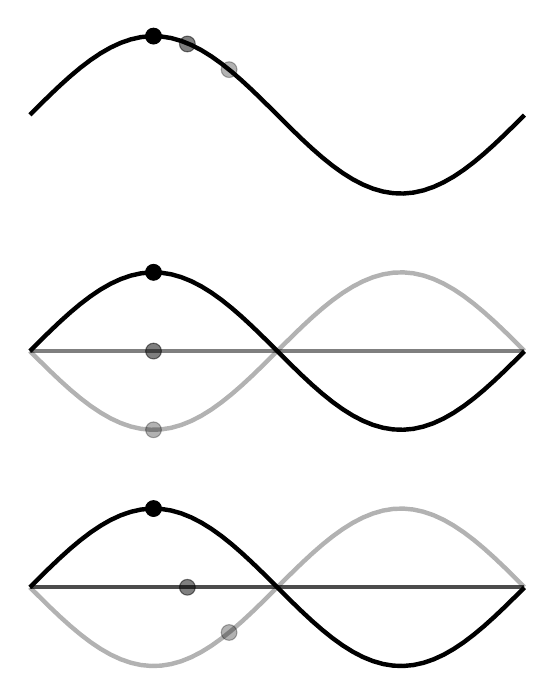
\begin{tikzpicture}
%\draw[help lines] (0,0) grid (2,3);
%\draw[step=0.5, gray, very thin] (-1.4,-1.4) grid (1.4,1.4);
%\draw (0,0) parabola (1,1.5) parabola[bend at end] (2,0);
%\draw (0,0) sin (1,1) cos (2,0) sin (3,-1) cos (4,0) sin (5,1);
%\draw [domain=0.5:1.25, samples=50] plot (\x, {0.1+sin(\x r)});
%\draw [green, dashed, domain=0:2*3.14, samples=50] plot (\x, {sin(\x r)});
\draw [ultra thick,domain=0:2*3.14, samples=50] plot (\x, {+sin(\x r)});
\draw [ultra thick,domain=0:2*3.14, samples=50,opacity=0.5] plot (\x, {0});
\draw [ultra thick,domain=0:2*3.14, samples=50,opacity=0.3] plot (\x, {-sin(\x r)});

\draw[fill=black] (3.14*0.5,1,0) circle (0.1 );
\draw[fill=black,opacity=0.5] (3.14*0.5,0,0) circle (0.1 );
\draw[fill=black,,opacity=0.3] (3.14*0.5,-1,0) circle (0.1 );



%\draw[help lines] (0,0) grid (2,3);
%\draw[step=0.5, gray, very thin] (-1.4,-1.4) grid (1.4,1.4);
%\draw (0,0) parabola (1,1.5) parabola[bend at end] (2,0);
%\draw (0,0) sin (1,1) cos (2,0) sin (3,-1) cos (4,0) sin (5,1);
%\draw [domain=0.5:1.25, samples=50] plot (\x, {0.1+sin(\x r)});
%\draw [green, dashed, domain=0:2*3.14, samples=50] plot (\x, {sin(\x r)});
\draw [ultra thick,domain=0:2*3.14, samples=50] plot (\x, {3+sin(\x r)});
%\draw [ultra thick,domain=0:2*3.14, samples=50,opacity=0.7] plot (\x, {0});
%\draw [ultra thick,domain=0:2*3.14, samples=50,opacity=0.3] plot (\x, {-sin(\x r)});

\draw[fill=black] (3.14*0.5,3+1,0) circle (0.1 );
\draw[fill=black,opacity=0.5] (2,3+0.9,0) circle (0.1 );
\draw[fill=black,,opacity=0.3] (2.53,3+0.574,0) circle (0.1 );

%\draw[help lines] (0,0) grid (2,3);
%\draw[step=0.5, gray, very thin] (-1.4,-1.4) grid (1.4,1.4);
%\draw (0,0) parabola (1,1.5) parabola[bend at end] (2,0);
%\draw (0,0) sin (1,1) cos (2,0) sin (3,-1) cos (4,0) sin (5,1);
%\draw [domain=0.5:1.25, samples=50] plot (\x, {0.1+sin(\x r)});
%\draw [green, dashed, domain=0:2*3.14, samples=50] plot (\x, {sin(\x r)});
\draw [ultra thick,domain=0:2*3.14, samples=50] plot (\x, {-3+sin(\x r)});
\draw [ultra thick,domain=0:2*3.14, samples=50,opacity=0.7] plot (\x, {-3});
\draw [ultra thick,domain=0:2*3.14, samples=50,opacity=0.3] plot (\x, {-3-sin(\x r)});

\draw[fill=black] (3.14*0.5,-3+1,0) circle (0.1 );
\draw[fill=black,opacity=0.5] (2,-3,0) circle (0.1 );
\draw[fill=black,,opacity=0.3] (2.53,-3-0.574,0) circle (0.1 );

 \end{tikzpicture}

 
\end{document}